\chapter{The Chernobyl Accident}
\label{ch:chernobyl}

On 26~April 1986, at 01:23:40 local time, an operator at Chernobyl Unit~4 pressed
the AZ-5 emergency shutdown button. Within seconds the reactor power surged to
many times its rated value, two explosions destroyed the core and building, and
the worst nuclear accident in history began. This chapter reconstructs the
sequence with the physics of the preceding chapters in hand. The aim is not to
assign blame but to show the equations playing out in a real machine.

\section{The test and its purpose}

The accident occurred during a \emph{safety test}, ironically intended to improve
the plant's response to a station blackout. The test sought to verify that, after a
loss of off-site power, the rotational inertia of a coasting-down turbine
generator could power the main coolant pumps for the brief interval before the
diesel generators reached full load. It was an electrical-engineering test of
turbine coastdown, to be run at reduced reactor power. Crucially, conducting it
required putting the reactor into a low-power state and disabling several
protective systems---taking the machine toward the corner of its operating
envelope where, as Chapter~\ref{ch:rbmk} showed, it was least stable.

\section{The descent into the unstable regime}

The test was planned for the daytime crew but was repeatedly delayed; the grid
dispatcher requested that Unit~4 keep supplying power through the evening. The
power reduction was thus stretched over many hours, during which two destabilising
processes unfolded.

\emph{Power reduction and xenon buildup.} The reactor was held at reduced power and
then, around 00:28, its thermal power fell far below the test plan---to roughly
$30\unit{MW}$ thermal, a small fraction of the $3200\unit{MW}$ rating. Accounts
differ on whether this was an operator control error or an instrumentation/control
fault; either way, the low power had a fateful consequence. During the preceding
hours at higher power the core had accumulated $^{135}$I; now, at very low flux,
xenon burnup ceased while iodine kept decaying into xenon
(Chapter~\ref{ch:xenon}). The core became heavily \textbf{xenon-poisoned}, and the
power could not easily be raised.

\emph{Rod withdrawal and loss of margin.} To fight the xenon and bring the power
back up for the test, operators withdrew control rods---many of them. By the time
power was coaxed to about $200\unit{MW}$ thermal (still well below the planned
$700\!-\!1000\unit{MW}$), the \textbf{operating reactivity margin} had fallen far
below its minimum, to the equivalent of only a handful of rods. The reactor was now
held critical by very few absorbers, with most withdrawn---the precise state in
which the void coefficient was largest, the axial flux shape distorted, and the
shutdown capability hollowed out.

\begin{figure}[H]
\centering
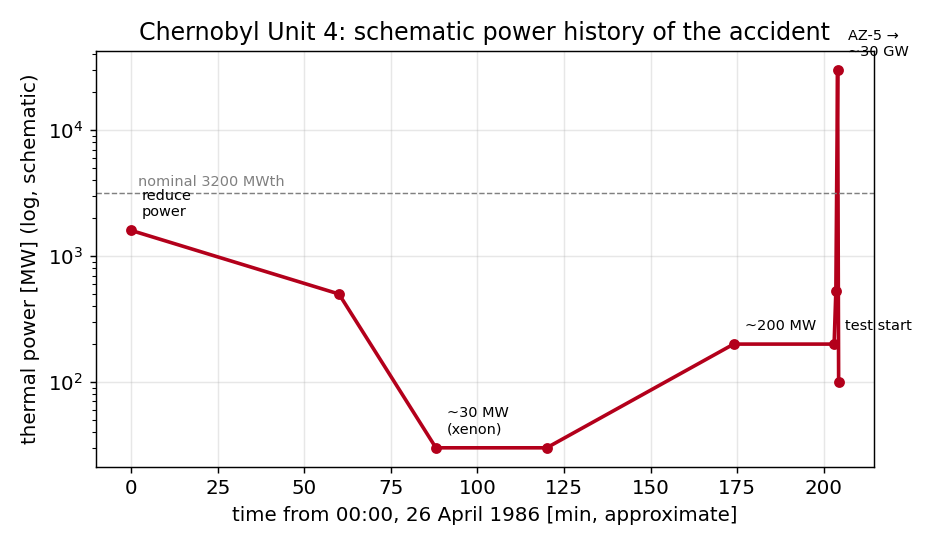
\includegraphics[width=0.92\linewidth]{figures/chernobyl_timeline.png}
\caption{Schematic thermal-power history of Chernobyl Unit~4 through the night of
the accident (illustrative, log scale). Power was reduced for the test, collapsed
to $\sim 30\unit{MW}$ with xenon poisoning, was partially recovered to
$\sim 200\unit{MW}$ by withdrawing rods, and then surged to tens of gigawatts in
seconds after AZ-5 was pressed.}
\label{fig:cher-timeline}
\end{figure}

\section{Starting the test}

With the reactor at about $200\unit{MW}$, the crew proceeded with the test rather
than aborting---a low power at which the RBMK's instability was acute. To run the
test they configured the plant in ways that further reduced safety margins:
additional main coolant pumps were running (increasing core flow, reducing
boiling and thus the steam void fraction, but pushing pumps toward cavitation),
and several automatic protection signals---including those that would have scrammed
the reactor on low water level or on the trip of the turbine---were blocked so that
the test would not be interrupted.

At 01:23:04 the turbine steam supply was closed to begin the coastdown. As the
main pumps driven by the coasting turbine slowed, core coolant flow decreased.
Less flow meant more boiling in the channels; more boiling meant more steam
\emph{voids}; and because the void coefficient was strongly positive, the voids
added reactivity. Power began to climb. In a negative-void reactor this would have
been self-correcting; in the RBMK it was self-amplifying. The reactor was now
sliding up the positive-feedback ramp.

\section{AZ-5 and the power surge}

At 01:23:40, with power rising, an operator pressed \textbf{AZ-5}, the emergency
scram, to insert all control and protection rods. What should have shut the
reactor down did the opposite---at first. As the rods began to descend from their
nearly fully-withdrawn positions, the \emph{graphite displacers} entered the lower
core first, displacing water (an absorber) and \textbf{adding} positive reactivity
in the bottom of the core (the positive scram effect of Chapter~\ref{ch:rbmk}).
Because the flux was already distorted toward the bottom of the core, this local
positive insertion struck exactly where it would do the most harm.

The added reactivity pushed the reactor through prompt criticality. Now the
physics of Chapters~\ref{ch:pk} and~\ref{ch:nonlinear} took over on the
millisecond timescale. With $\rho>\beta$, the power grew as
$\exp[(\rho-\beta)t/\Lambda]$; the positive void feedback, far from arresting the
rise, reinforced it as the surging power flashed the remaining water to steam; and
there was no sufficient prompt negative feedback to cap the excursion. The power
spiked to an estimated tens of gigawatts---perhaps a hundred times the rated
power---in a few seconds.

\section{The explosions}

The energy deposited in this prompt excursion was enormous and almost
instantaneous. The fuel overheated and fragmented; the intense heat flashed the
cooling water to steam, and the pressure surge ruptured fuel channels. The first
explosion was a \textbf{steam explosion}---the violent expansion of suddenly
generated steam---which blew off the $1000$-tonne upper biological shield
(``Elena'') and tore open the core. A second explosion followed seconds later;
its exact nature is debated (a further steam/thermal explosion, possibly with a
contribution from hydrogen generated by steam reacting with hot zirconium and
graphite, and a brief renewed criticality in the disrupted core). The explosions
demolished the reactor hall, ejected fuel and graphite, and exposed the core to
the atmosphere.

\section{The fire and the release}

With the core breached and the graphite moderator exposed to air at high
temperature, the \textbf{graphite caught fire}. The fire burned for days, lofting
fission products---$^{131}$I, $^{137}$Cs, $^{134}$Cs, and others---high into the
atmosphere, where winds carried them across the western Soviet Union and Europe.
The decay heat (Chapter~\ref{ch:decay}) in the wrecked fuel sustained high
temperatures and continued to drive releases. Emergency crews fought the fire and
later dropped boron, sand, clay, and lead from helicopters in an attempt to
smother the core and absorb neutrons. The release continued for about ten days
before subsiding.

\section{The sequence in one paragraph}

Stripped to essentials: a delayed, low-power test poisoned the core with xenon;
fighting the xenon stripped out the control rods, leaving the reactor in its most
unstable configuration with almost no shutdown margin; reducing coolant flow for
the test boiled more water, and the positive void coefficient drove power upward;
the emergency scram, through the graphite-tipped rods, added reactivity instead of
removing it and pushed the reactor prompt-critical; the positive void feedback
amplified the prompt excursion; and the resulting energy surge flashed the coolant
and exploded the core. Every step is a chapter of this book made flesh. The next
chapter analyses why, and how the understanding evolved.


\section*{Exercises}
\addcontentsline{toc}{section}{Exercises}
\begin{enumerate}[leftmargin=*,itemsep=2pt]
\item Reconstruct the chain of events from the power drop to the explosions in five steps.
\item Explain why reducing coolant flow for the test raised reactor power.
\item Why did pressing AZ-5 initially increase reactivity?
\item Estimate, qualitatively, why the excursion was over in seconds using the prompt timescale.
\item Distinguish the roles of the steam explosion and the graphite fire in the consequences.
\end{enumerate}
